\documentclass[12pt]{article}
\usepackage[utf8]{inputenc}  
\usepackage[english]{babel}
\usepackage{amsmath, amssymb, amsfonts}
\usepackage{authblk}
\usepackage{booktabs}
\usepackage{array}
\usepackage{caption}
\usepackage{subcaption}
\usepackage{algorithm}
\usepackage{algpseudocode}
\usepackage{hyphenat}
\usepackage{xcolor}
\usepackage{listings}        
\usepackage{microtype}
\usepackage{graphicx}
\usepackage[hidelinks]{hyperref}
\usepackage{geometry}
\usepackage{doi}
\setlength{\emergencystretch}{2em}
\renewcommand{\doitext}{doi:\penalty0\ }
\geometry{margin=1in}

% Colors for listings
\definecolor{codebg}{rgb}{0.95,0.95,0.97}
\definecolor{frameworkblue}{RGB}{10,40,80}
\lstset{
    language=Python,
    basicstyle=\ttfamily\footnotesize,
    backgroundcolor=\color{codebg},
    frame=single,
    rulecolor=\color{frameworkblue},
    breaklines=true,
    showstringspaces=false,
    commentstyle=\color{green!60!black}\itshape,
    keywordstyle=\color{frameworkblue}\bfseries,
    stringstyle=\color{red!70!black},
    numbers=left,
    numberstyle=\tiny\color{gray},
    numbersep=6pt,
    tabsize=4,
    captionpos=b
}

% Useful commands
\newcommand{\R}{\mathbb{R}}
\newcommand{\M}{\mathbf{M}}
\newcommand{\K}{\mathbf{K}}
\newcommand{\A}{\mathcal{A}}
\newcommand{\Rstate}{\mathbf{R}}
\newcommand{\trans}{^{\mathsf{T}}}

\title{A Unified Structural and Operator Framework \\ for the Linear $n$-Mass Pendulum}
\author[1]{Yonatan Ali Rodr\'iguez Arias\thanks{\texttt{yonatanorion\_84@hotmail.com}}}
\author[1]{Sandra Arellano Gonz\'alez\thanks{\texttt{ag.sandra012@gmail.com}}}
% Afiliación (la misma para los tres)
\affil[1]{Escuela Superior de Ingenier\'ia Mec\'anica y El\'ectrica 
         Unidad Profesional ``Adolfo L\'opez Mateos'' Building 5, 3rd floor, 
         Zacatenco, Delegaci\'on Gustavo A. Madero, Ciudad de M\'exico, 07738}
% Fecha
\date{July 2026}
\begin{document}
\maketitle
\begin{abstract}
\noindent A computational framework is presented that bridges the symbolic generation and linear dynamic propagation of the $n$-mass pendulum. The core contribution is the identification of a structural cumulative mass-sum rule that naturally governs the inertial, coupling, and gravitational terms derived from Lagrange's equations. This universal organizing principle eliminates the need for manual or recursive indexing, yielding a compact, explicit matrix assembly algorithm for arbitrary $n$.

The assembled linear system is solved both by standard modal decoupling and in state-space form.  The latter is propagated with a scaled-and-squared truncated Peano--Baker (Taylor) series for the matrix exponential.  The framework is intentionally limited to the linear regime, where both implementations agree with a reference matrix exponential to double-precision round-off. Because the transition matrix is constant for fixed parameters and timestep, it can be precomputed once and reused efficiently across repeated simulations, parameter sweeps, or control evaluations.

A brief discussion records the variation-of-constants representation for a possible nonlinear extension and points to modern exponential integrators; a full nonlinear method is outside the scope of this work. The proposed pipeline offers pedagogical transparency and explicit structural mapping, serving as a unified bridge between symbolic multibody generation and linear solution strategies.
\end{abstract}

\noindent\textbf{Keywords:} Multi-body Dynamics, $n$-mass Pendulum, Structural Generation, Linear State-Space, Matrix Exponential, Peano-Baker Series

\section{Introduction}

The pendulum remains one of the most fundamental systems in classical mechanics and continues to serve as a canonical model in multibody dynamics, robotics, vibration analysis, and control systems~\cite{lobas2005generalized,fritzkoski2008dynamics,fritzkoski2009dynamics,pieranski2005dynamics,kawaji1991control,raymond2013pendulum}. While the equations of motion for single and double pendulum systems are widely known, explicitly deriving the equations governing an arbitrary $n$-mass pendulum rapidly becomes cumbersome due to the combinatorial growth of inertial and trigonometric coupling terms.

\subsection{Related Work and Framework Positioning}

Several mature approaches exist for multibody equation generation and simulation. Featherstone's articulated-body algorithm~\cite{featherstone2008rigid} prioritizes recursive computational efficiency, achieving $\mathcal{O}(n)$ scaling suitable for real-time applications, though it operates implicitly through factorized spatial algebra. Kane's method~\cite{kane1985dynamics} provides a highly systematic approach for deriving minimal-order equations but typically requires manual formulation for specific topologies. General recursive formulations covering serial and tree-topology systems are treated in~\cite{jain2010robot,shabana2010dynamics}. Furthermore, general-purpose symbolic environments (e.g., SymPy mechanics) can derive explicit equations but often yield massive, unstructured expressions for large $n$.

The present work pursues a different and complementary objective: \textbf{explicit structural transparency}. Instead of focusing on raw computational speed for massive degrees of freedom, the main contribution is the identification of a cumulative mass-sum pattern that acts as a universal algebraic organizing principle throughout the linearized equations of motion.

The resulting symmetric positive-definite second-order system admits the standard generalized-eigenvalue (modal) solution.  We use that solution as an independent reference and retain a state-space matrix-exponential implementation for applications in which a transition operator is convenient, such as control and repeated propagation.  The matrix exponential is evaluated by a scaled-and-squared truncated Peano--Baker (Taylor) series; this numerical device is standard and is not claimed as a new matrix-exponential algorithm. The conceptual pipeline is illustrated in Figure~\ref{fig:pipeline}.

\begin{figure}[htbp]
  \centering
  \vspace{0.3cm}
  \noindent\fbox{%
    \parbox{0.95\textwidth}{%
      \centering
      \vspace{0.2cm}
      \textbf{Lagrangian Formulation} $\longrightarrow$
      \textbf{Cumulative Mass-Sum Rule} $\longrightarrow$
      \textbf{Matrix Assembly} \\ \vspace{0.2cm}
      $\longrightarrow$ \textbf{State-Space Linearization} $\longrightarrow$
      \textbf{Matrix Exponential Propagation}
      \vspace{0.2cm}
    }%
  }
  \vspace{0.2cm}
  \caption{Conceptual pipeline of the proposed framework, bridging explicit structural generation and operator-based linear propagation.}
  \label{fig:pipeline}
\end{figure}

The paper is organized as follows. Sections 2--4 develop the symbolic generation framework and introduce the cumulative mass-sum rule. Sections 5--6 derive the state-space system and the operator-based propagator. Section 7 presents validation results in the linear regime. Section 8 briefly outlines a possible nonlinear extension (as a proof of concept) and delimits it as future work. Finally, Section 9 concludes.

\section{Lagrangian Formulation of the \texorpdfstring{$n$}{n}-Mass Pendulum}
\label{sec:lagrangian}

\subsection{Equations of Motion}

The dynamics of the system are derived from the Euler-Lagrange equations
\begin{equation}\label{eq:euler-lagrange}
  \frac{d}{dt}\left(\frac{\partial L}{\partial \dot{q}_j}\right)
  - \frac{\partial L}{\partial q_j} = 0,
\end{equation}
where the Lagrangian is defined as $L = T - U$, with $T$ the kinetic energy and $U$ the potential energy. For the $n$-mass pendulum,
\[
T = \frac{1}{2} \sum_{i=1}^{n} m_i v_i^2, \qquad
U = g \sum_{i=1}^{n} m_i y_i,
\]
and $v_i^2 = \dot{x}_i^2 + \dot{y}_i^2$.  The generalized coordinates are $q_j = \theta_j$, $j=1,\dots,n$.

\subsection{Coordinate Convention}

Each generalized coordinate $\theta_i$ is measured with respect to the downward vertical direction, as illustrated in Figure~\ref{fig:n_mass}.  The Cartesian coordinates of the $i$-th mass are therefore
\begin{align}
  x_i &= \sum_{k=1}^{i} l_k \sin\theta_k, \label{eq:xi} \\
  y_i &= -\sum_{k=1}^{i} l_k \cos\theta_k. \label{eq:yi}
\end{align}
The origin is taken at the pivot, with the positive $x$-axis to the right and the positive $y$-axis upward.  This convention ensures that when all $\theta_k = 0$ (vertical downward equilibrium), $y_i = -\sum_{k=1}^i l_k$ and $x_i=0$.

\begin{figure}[htbp]
  \centering
  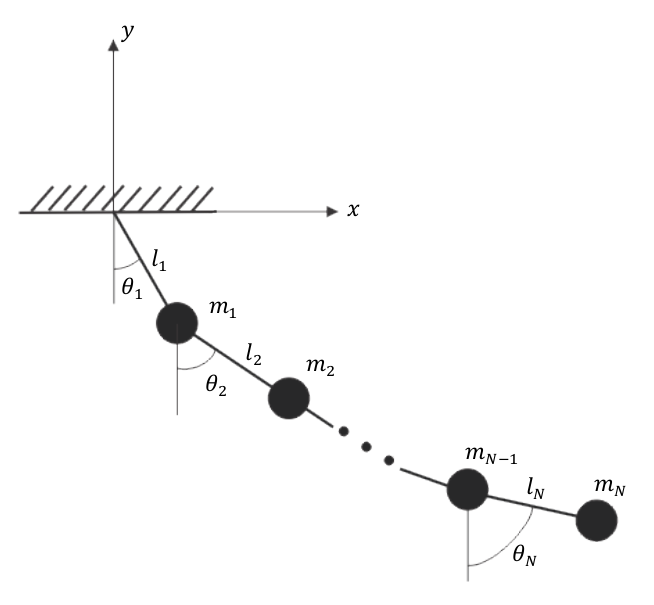
\includegraphics[width=0.6\textwidth]{figures/n_mass_pendulum.png}
  \caption{General $n$-mass pendulum with the absolute joint angle convention. Each angle $\theta_i$ is measured from the downward vertical. The coordinate origin is at the pivot.}
  \label{fig:n_mass}
\end{figure}

\subsection{Explicit Derivation of Kinetic Energy}

Differentiating Eqs.~(\ref{eq:xi}) and (\ref{eq:yi}) with respect to time gives the velocity components:
\begin{align}
  \dot{x}_i &= \sum_{k=1}^{i} l_k \dot{\theta}_k \cos\theta_k, \\
  \dot{y}_i &= \sum_{k=1}^{i} l_k \dot{\theta}_k \sin\theta_k.
\end{align}
Hence,
\begin{equation}
  v_i^2 = \dot{x}_i^2 + \dot{y}_i^2 = 
  \sum_{k=1}^{i}\sum_{r=1}^{i} l_k l_r \dot{\theta}_k \dot{\theta}_r
  \bigl(\cos\theta_k\cos\theta_r + \sin\theta_k\sin\theta_r\bigr).
\end{equation}
Using the trigonometric identity $\cos\theta_k\cos\theta_r+\sin\theta_k\sin\theta_r = \cos(\theta_k-\theta_r)$, we obtain the compact expression
\begin{equation}\label{eq:v_sq}
  v_i^2 = \sum_{k=1}^{i}\sum_{r=1}^{i}
  l_k l_r \dot{\theta}_k \dot{\theta}_r
  \cos(\theta_k-\theta_r).
\end{equation}
Note that the double sum runs over all pairs of links up to the $i$-th mass.  The total kinetic energy is then
\begin{equation}
  T = \frac{1}{2} \sum_{i=1}^{n} m_i \sum_{k=1}^{i}\sum_{r=1}^{i}
  l_k l_r \dot{\theta}_k \dot{\theta}_r \cos(\theta_k-\theta_r).
\end{equation}

\subsection{Potential Energy and its Linearization}

Substituting $y_i$ from Eq.~(\ref{eq:yi}) gives the potential energy
\begin{equation}
  U = g \sum_{i=1}^{n} m_i \left(-\sum_{k=1}^{i} l_k \cos\theta_k\right)
  = -g \sum_{k=1}^{n} \left(\sum_{i=k}^{n} m_i\right) l_k \cos\theta_k.
\end{equation}
For small oscillations we expand $\cos\theta_k \approx 1 - \theta_k^2/2$; the constant term does not affect the dynamics, so the relevant part is
\begin{equation}\label{eq:U_quadratic}
  U_{\text{quad}} = \frac{g}{2} \sum_{k=1}^{n} \left(\sum_{i=k}^{n} m_i\right) l_k \theta_k^2.
\end{equation}
No cross terms $\theta_i\theta_j$ ($i\neq j$) appear because the expansion of each cosine depends only on its own angle.  This crucial simplification leads to a diagonal stiffness matrix, as shown in Section~\ref{sec:diagonal}.

\section{Structural Pattern of the Equations of Motion}
\label{sec:structural}

For small systems, the equations of motion can be derived manually.  However, the combinatorial growth of velocity products makes manual derivation impractical for large $n$.  Inspection of systems with $n \in \{1, 2, 3, 4\}$ reveals a clear invariant structural property: every term in the $d$-th equation that involves coordinate $\theta_k$ or its derivatives contains the factor
\begin{equation}\label{eq:prefix-sum}
  \boxed{M_{d,k}^{\mathrm{coeff}} = \sum_{i=\max(d,k)}^{n} m_i}.
\end{equation}

\subsection{The Cumulative Mass-Sum Rule as an Organizing Principle}

This quantity represents the effective inertia dynamically shared by joints $d$ and $k$.  It acts as a universal organizing principle because the identical cumulative structure governs:
\begin{itemize}
  \item diagonal and coupled acceleration terms,
  \item centrifugal and Coriolis-like velocity-squared terms,
  \item localized gravitational contributions.
\end{itemize}

Physical interpretation: when $k \ge d$, joint $d$ contributes to the acceleration of all masses extending from coordinate $k$ to the end of the chain.  Conversely, when $k < d$, the inertial coupling relies on the deeper segment of the chain.

\subsection{Explicit Example for \texorpdfstring{$n=4$}{n=4}}

Applying the rule to the four-mass pendulum yields the first equation ($d=1$), noting the proper dimensionality factor $l_1$:
\begin{align}
  &(m_1+m_2+m_3+m_4)l_1^2\ddot{\theta}_1
  + (m_2+m_3+m_4)l_1 l_2\ddot{\theta}_2\cos(\theta_1-\theta_2) \nonumber \\
  &+ (m_3+m_4)l_1 l_3\ddot{\theta}_3\cos(\theta_1-\theta_3)
  + m_4 l_1 l_4\ddot{\theta}_4\cos(\theta_1-\theta_4) \nonumber \\
  &+ (m_2+m_3+m_4)l_1 l_2\dot{\theta}_2^2\sin(\theta_1-\theta_2)
  + (m_3+m_4)l_1 l_3\dot{\theta}_3^2\sin(\theta_1-\theta_3) \nonumber \\
  &+ m_4 l_1 l_4\dot{\theta}_4^2\sin(\theta_1-\theta_4)
  + (m_1+m_2+m_3+m_4)g l_1\sin\theta_1 = 0 \label{eq:j1}
\end{align}
and the second equation ($d=2$), scaled by $l_2$:
\begin{align}
  &(m_2+m_3+m_4)l_2^2\ddot{\theta}_2
  + (m_3+m_4)l_2 l_3\ddot{\theta}_3\cos(\theta_2-\theta_3)
  + m_4 l_2 l_4\ddot{\theta}_4\cos(\theta_2-\theta_4) \nonumber \\
  &+ (m_2+m_3+m_4)l_1 l_2\ddot{\theta}_1\cos(\theta_1-\theta_2)
  + (m_3+m_4)l_2 l_3\dot{\theta}_3^2\sin(\theta_2-\theta_3) \nonumber \\
  &+ m_4 l_2 l_4\dot{\theta}_4^2\sin(\theta_2-\theta_4)
  - (m_2+m_3+m_4)l_1 l_2\dot{\theta}_1^2\sin(\theta_1-\theta_2) \nonumber \\
  &+ (m_2+m_3+m_4)g l_2\sin\theta_2 = 0. \label{eq:j2}
\end{align}
The third and fourth equations can be obtained using the same methodology. 
Every coefficient is exactly a cumulative mass sum: $\sum_{i=\max(d,k)}^n m_i$ multiplied by the product of lengths $l_d l_k$.

\section{Algorithmic Generation Framework}
\label{sec:generation}

The complete symbolic structure can be mapped into a concise algorithm using the mass-sum rule, eliminating complex parsers or manual recursion.

\subsection{Matrix Assembly from the Cumulative Sums}

We define the mass matrix $\M(\boldsymbol{\theta})$ and the Coriolis/centrifugal vector $\mathbf{c}(\boldsymbol{\theta},\dot{\boldsymbol{\theta}})$ through the relation
\[
\M(\boldsymbol{\theta})\ddot{\boldsymbol{\theta}} + \mathbf{c}(\boldsymbol{\theta},\dot{\boldsymbol{\theta}}) + \mathbf{g}(\boldsymbol{\theta}) = \mathbf{0},
\]
where $\mathbf{g}(\boldsymbol{\theta})$ is the gravitational torque vector.  The cumulative mass-sum rule gives explicit formulas:
\begin{align}
M_{jk}(\boldsymbol{\theta}) &= \left(\sum_{i=\max(j,k)}^{n} m_i\right) l_j l_k \cos(\theta_j-\theta_k), \\
c_d(\boldsymbol{\theta},\dot{\boldsymbol{\theta}}) &=
\sum_{k=1}^{n} \left(\sum_{i=\max(d,k)}^{n} m_i\right) l_d l_k \,
\dot{\theta}_k^2 \sin(\theta_d-\theta_k), \\
g_d(\boldsymbol{\theta}) &= \left(\sum_{i=d}^{n} m_i\right) g l_d \sin\theta_d.
\end{align}
The sine difference alone determines the sign of every velocity-squared term; no additional index-dependent sign is present.  For example, when $d=2$ and $k=1$, $\sin(\theta_2-\theta_1)=-\sin(\theta_1-\theta_2)$, exactly as in Eq.~(\ref{eq:j2}).
For the linearized case (small angles) we set $\cos(\cdot)=1$, $\sin(\cdot)=0$ except in the gravitational term where $\sin\theta_d\approx\theta_d$.

\subsection{Algorithm for Linear System Assembly}

The following algorithm constructs the linearized system matrices directly from the cumulative sums without symbolic differentiation.

\begin{algorithm}[htbp]
  \caption{Linear Matrix Assembly via Cumulative Mass-Sum Rule}
  \label{alg:assembly}
  \begin{algorithmic}[1]
    \Require masses $m_1,\ldots,m_n$, lengths $l_1,\ldots,l_n$, $g$
    \Ensure mass matrix $\M$, stiffness matrix $\K$
    \State $S_n \gets m_n$
    \For{$j \gets n-1$ \textbf{down to} $1$}
      \State $S_j \gets m_j + S_{j+1}$
    \EndFor
    \For{$j \gets 1$ \textbf{to} $n$}
      \For{$k \gets 1$ \textbf{to} $n$}
        \State $M_{jk} \gets S_{\max(j,k)} l_j l_k$
      \EndFor
      \State $K_{jj} \gets S_j g l_j$
    \EndFor
  \end{algorithmic}
\end{algorithm}

\subsection{Algorithmic Scaling}

The suffix masses $S_j$ require $\mathcal{O}(n)$ work and are computed once.  The subsequent loop assigns $n^2$ entries of $\M$ and $n$ nonzero entries of $\K$, so the assembly requires $\mathcal{O}(n^2)$ work and storage.  Recomputing the sum $\sum_{i=\max(j,k)}^n m_i$ inside every matrix entry would instead require $\mathcal{O}(n^3)$ work and is deliberately avoided.

\begin{table}[htbp]
  \centering
  \caption{Number of entries assigned by the linear matrix assembly.}
  \label{tab:scaling-generation}
  \begin{tabular}{cccc}
    \toprule
    $n$ & Entries of $\M$ & Nonzero entries of $\K$ & Total \\
    \midrule
    2 & 4 & 2 & 6 \\
    4 & 16 & 4 & 20 \\
    6 & 36 & 6 & 42 \\
    8 & 64 & 8 & 72 \\
    10 & 100 & 10 & 110 \\
    \bottomrule
  \end{tabular}
\end{table}

\section{Linearization and Matrix Assembly}
\label{sec:linearization}

\subsection{Small-Angle Approximation}

For small oscillations, we assume $|\theta_j| \ll 1$ rad.  The following approximations are applied:
\[
\sin\theta_j \approx \theta_j, \quad \cos(\theta_i-\theta_j) \approx 1,
\]
and velocity-squared terms (which are second order in small quantities) are neglected.  Under these assumptions the equations of motion reduce to the linear system
\begin{equation}
\M \ddot{\boldsymbol{\theta}} + \K \boldsymbol{\theta} = \mathbf{0},
\end{equation}
where $\M$ and $\K$ are constant matrices.

\subsection{Derivation of the Mass Matrix}

Inserting the small-angle approximation $\cos(\theta_j-\theta_k)\approx 1$ into the general expression for $M_{jk}(\boldsymbol{\theta})$ yields the constant mass matrix
\begin{equation}\label{eq:Mjk}
  M_{jk} = \left(\sum_{i=\max(j,k)}^{n} m_i\right) l_j l_k.
\end{equation}
Note that $M_{jk}=M_{kj}$ because $\max(j,k)=\max(k,j)$.  The matrix is symmetric and positive definite for positive masses and lengths.

\subsection{Diagonal Structure of the Gravitational Stiffness Matrix}
\label{sec:diagonal}

From the potential energy expansion (Eq.~(\ref{eq:U_quadratic})), the gravitational torque on joint $d$ is
\[
g_d = \frac{\partial U_{\text{quad}}}{\partial \theta_d}
= g \left(\sum_{i=d}^{n} m_i\right) l_d \theta_d.
\]
Therefore the stiffness matrix $\K$ is diagonal:
\begin{equation}\label{eq:Kjk}
  K_{jk} = \left(\sum_{i=j}^{n} m_i\right) g l_j \,\delta_{jk}.
\end{equation}
No off-diagonal entries appear because the quadratic potential contains only $\theta_j^2$ terms; the coordinate convention (angles measured from the downward vertical) eliminates $\theta_i\theta_j$ cross couplings.

\subsection{Standard Modal Decoupling}

Because $\M$ and $\K$ are symmetric positive definite for positive masses and lengths, the generalized eigenproblem admits an $\M$-orthonormal modal matrix $\mathbf{U}$:
\begin{equation}\label{eq:modal-eigenproblem}
  \K\mathbf{U}=\M\mathbf{U}\boldsymbol{\Omega}^{2},\qquad
  \mathbf{U}\trans\M\mathbf{U}=\mathbf{I},\qquad
  \mathbf{U}\trans\K\mathbf{U}=\boldsymbol{\Omega}^{2},
\end{equation}
where $\boldsymbol{\Omega}=\operatorname{diag}(\omega_1,\ldots,\omega_n)$ and $\omega_j>0$.  With $\boldsymbol{\theta}=\mathbf{U}\mathbf{q}$, the system decouples into $\ddot q_j+\omega_j^2q_j=0$, with the exact solution
\begin{equation}\label{eq:modal-solution}
  q_j(t)=q_j(0)\cos(\omega_j t)
  +\frac{\dot q_j(0)}{\omega_j}\sin(\omega_j t).
\end{equation}
This is the natural direct solution for the unforced linear second-order problem and is used below as an independent numerical reference.

\subsection{State-Space Representation}

Define the state vector $\Rstate(t) = (\boldsymbol{\theta}(t), \dot{\boldsymbol{\theta}}(t))\trans \in \R^{2n}$.  The linearized system can then be written as
\begin{equation}
\dot{\Rstate} = \A \Rstate, \qquad
\A = \begin{pmatrix}
\mathbf{0} & \mathbf{I} \\
-\M^{-1}\K & \mathbf{0}
\end{pmatrix}.
\end{equation}
The matrix $\A$ is constant, which allows the use of explicit operator-based propagators.  This first-order form is not required for the modal solution; it is retained because a reusable transition matrix is convenient in state-space control, forcing, and estimation workflows.

\section{Operator-Based Dynamic Propagation}
\label{sec:operator}

\subsection{Peano-Baker Series for the Transition Matrix}

Because $\A$ is constant, the state transition matrix from $0$ to $t$
is the matrix exponential $\Phi(t,0)=e^{\A t}$.

For the autonomous system considered here, the Peano--Baker series is
exactly the Taylor series of the matrix exponential.  A direct truncated
Taylor series can be inaccurate when $\|\A\Delta t\|$ is large
\cite{moler2003dubious}, so the implementation uses scaling and squaring.

A convenient implementation defines $\mathbf{X}=\A\Delta t$ and chooses
$s=\max\{0,\lceil\log_2(\|\mathbf{X}\|_{\infty}/\eta)\rceil\}$ with
$\eta=1/2$.  For $\mathbf{B}=\mathbf{X}/2^s$, the approximation is
\begin{equation}\label{eq:peano-truncated}
  \Phi(\Delta t) \approx
  \left(\sum_{k=0}^{N} \frac{\mathbf{B}^k}{k!}\right)^{2^s}.
\end{equation}
Scaling controls the Taylor remainder before repeated squaring.  With $N=20$, the tested systems agree with both \texttt{scipy.linalg.expm} and the modal solution to double-precision round-off.  This implementation is included for transparency; robust library routines based on established matrix-exponential algorithms should be preferred outside the tested parameter range.

\subsection{Propagation Algorithm and Reusability}

Once $\Phi(\Delta t)$ is precomputed (using the scaled series), the linear propagation over a time step is simply
\[
\Rstate(t+\Delta t) = \Phi(\Delta t) \Rstate(t).
\]
This requires only matrix-vector multiplications, making it highly efficient for repeated time stepping. Importantly, because $\Phi(\Delta t)$ is constant for fixed system parameters and time step, it can be precomputed once and reused across many simulations (e.g., parameter sweeps, Monte Carlo runs, or real-time control loops). This reusability is a key practical advantage of the operator-based formulation.

\section{Numerical Validation (Linear Regime)}
\label{sec:validation}

\subsection{Linear Validation}

To ensure a comprehensive evaluation and guarantee reproducibility, the linear framework was validated across four distinct test cases. In all scenarios, the gravitational acceleration was set to $g = 9.81$ m/s$^2$ and the systems were released from rest ($\dot{\boldsymbol{\theta}}(0) = \mathbf{0}$). The specific parameter sets--masses $m$ (in kg), lengths $l$ (in m), and initial angular displacements $\boldsymbol{\theta}(0)$ (in radians)--are defined as follows:
\begin{itemize}
  \item \textbf{$n=2$ (uniform):} $m_i = 1.0$, $l_i = 1.0$, and $\boldsymbol{\theta}(0) = [0.1, 0.05]\trans$.
  \item \textbf{$n=3$ (uniform):} $m_i = 1.0$, $l_i = 1.0$, and $\boldsymbol{\theta}(0) = [0.1, 0.05, 0.02]\trans$.
  \item \textbf{$n=3$ (non-uniform):} $m = [2.0, 1.5, 0.8]\trans$, $l = [1.2, 0.9, 0.6]\trans$, and $\boldsymbol{\theta}(0) = [0.1, 0.05, 0.02]\trans$.
  \item \textbf{$n=5$ (uniform):} $m_i = 1.0$, $l_i = 1.0$, and $\boldsymbol{\theta}(0) = [0.1, 0.05, 0.02, 0.01, 0.005]\trans$.
\end{itemize}

These configurations provide a baseline for verifying the assembly and propagation across varying dimensionalities and inertial distributions. The scaled Peano--Baker series was truncated at $N = 20$ with a time step of $\Delta t = 0.01$ s. Reference solutions were generated both by direct matrix exponentiation (\texttt{scipy.linalg.expm}) and by the generalized-eigenvalue solution in Eq.~(\ref{eq:modal-solution}).

\begin{figure}[htbp]
  \centering
  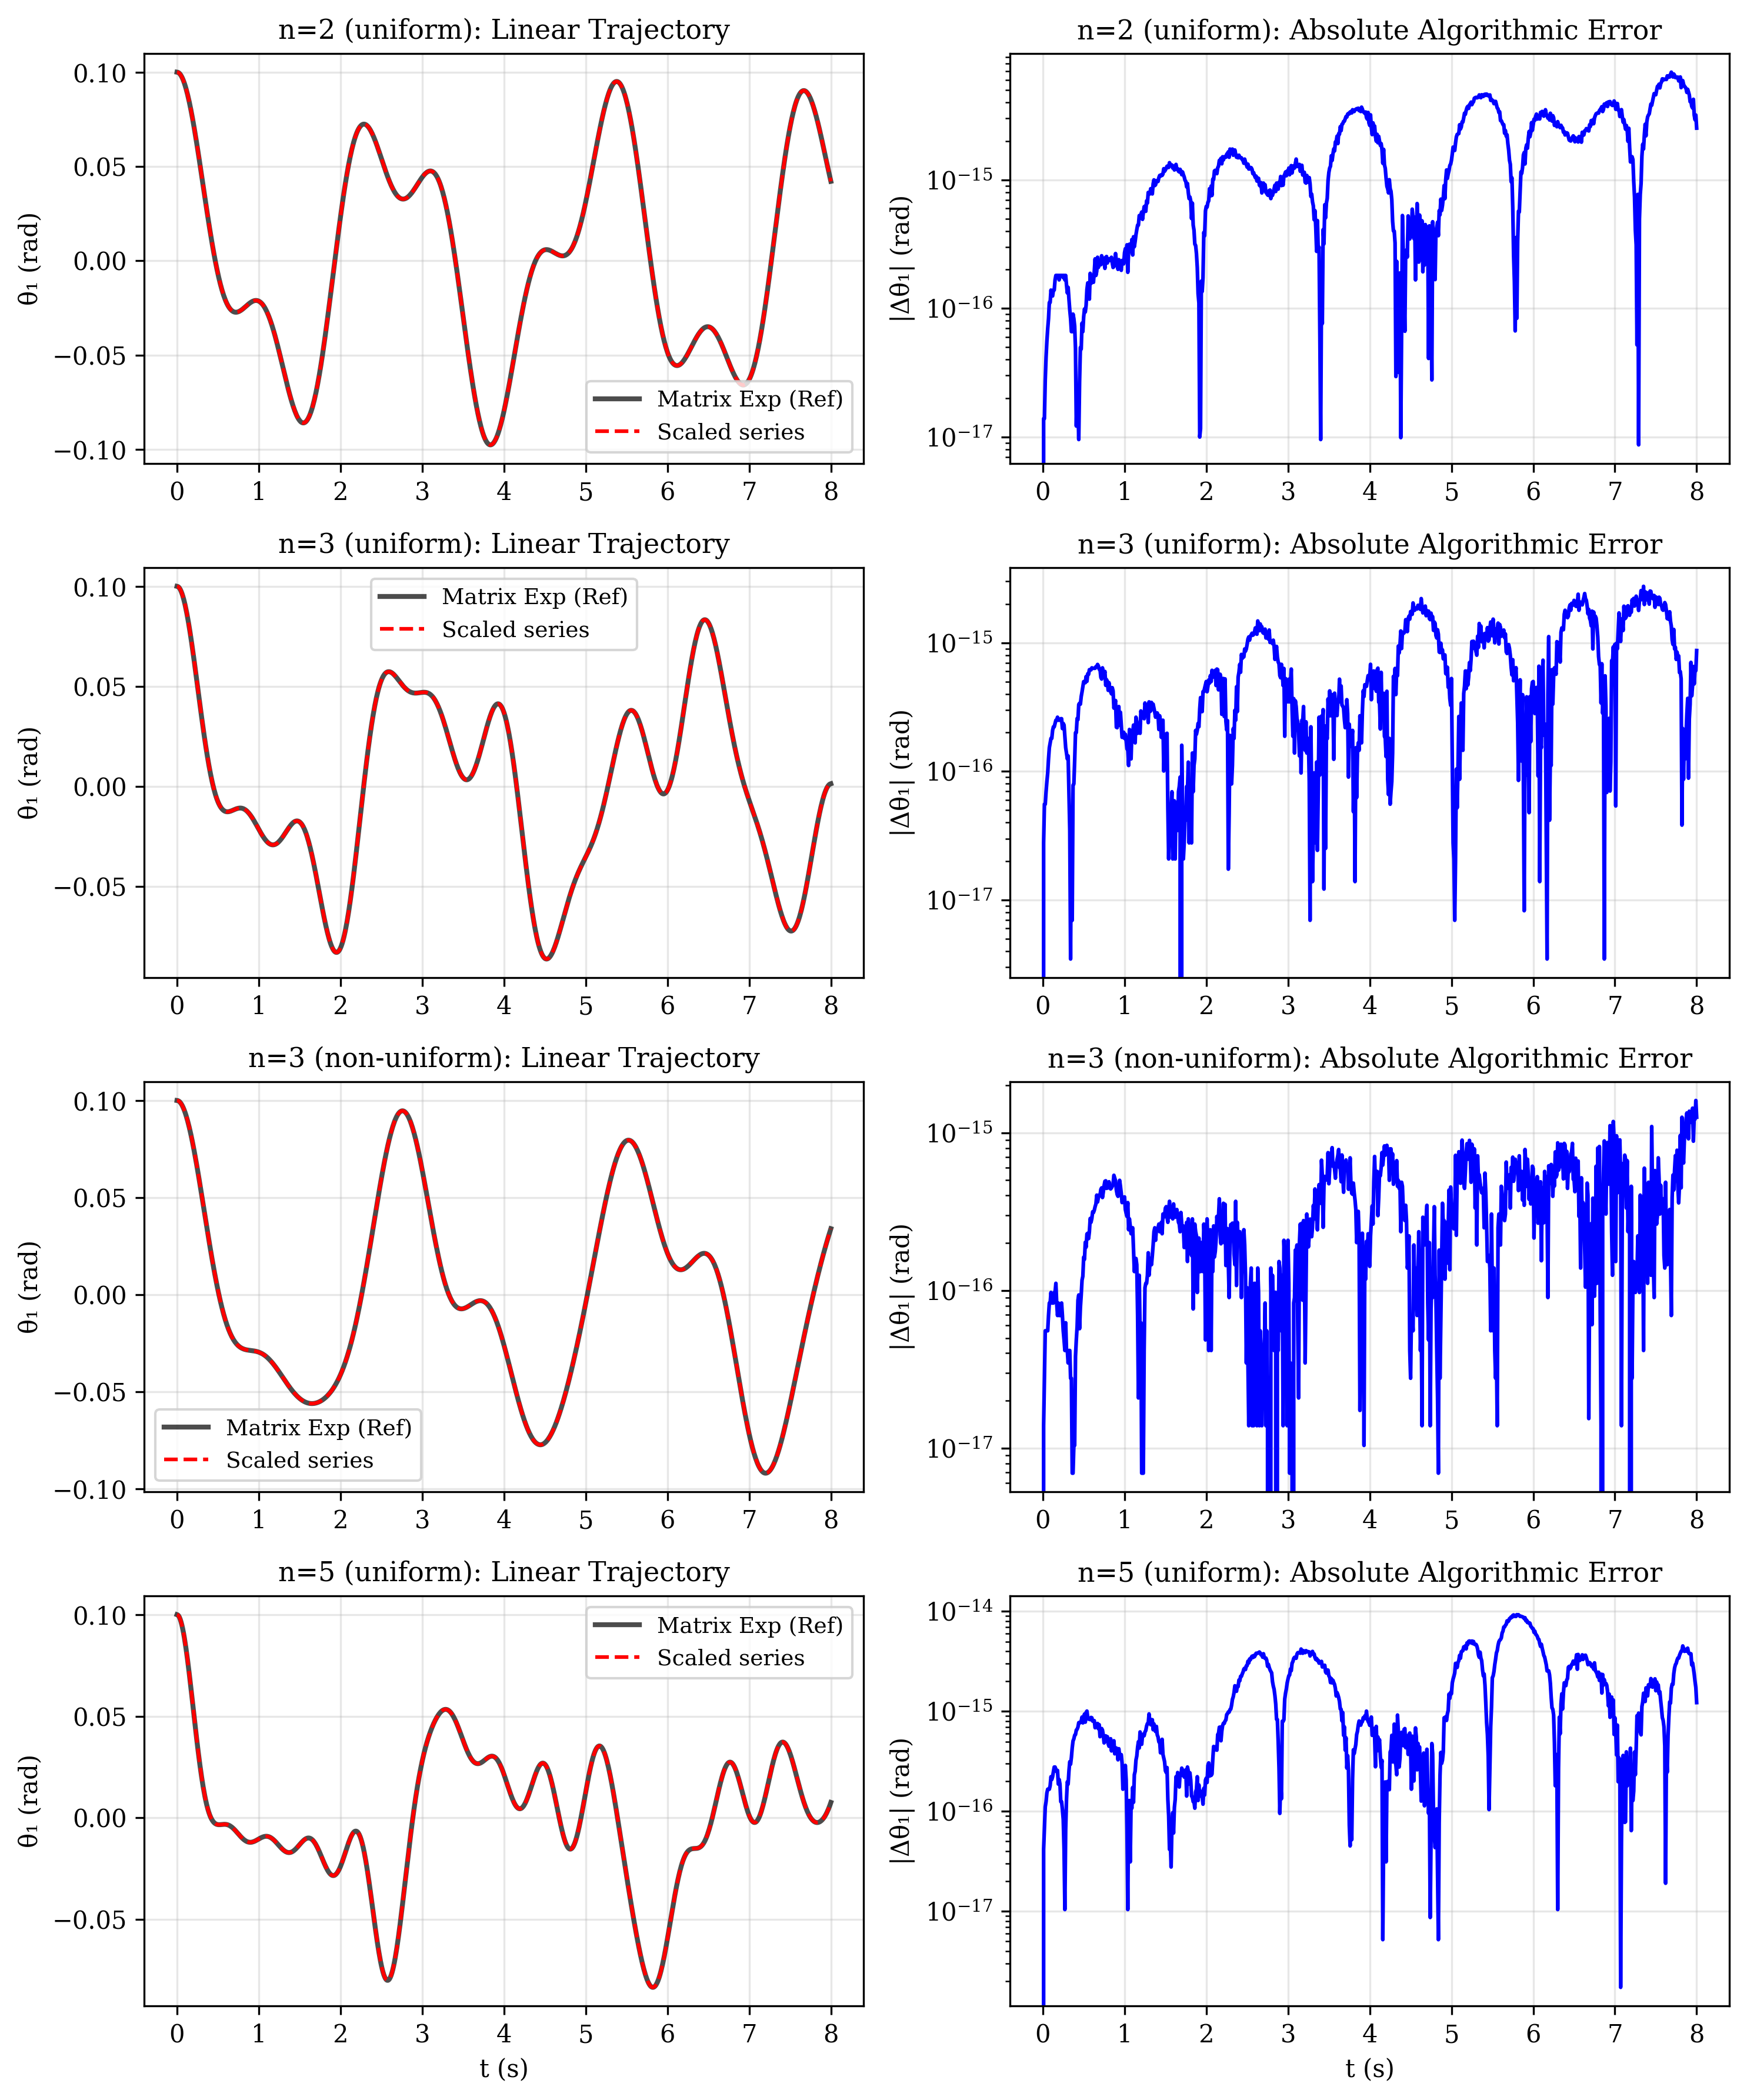
\includegraphics[width=0.8\textwidth]{figures/linear_validation.png}
  \caption{Linear validation results for the evaluated configurations. Left column: time-domain trajectories showing scaled-series stepping (dashed) versus the reference matrix exponential (solid). Right column: absolute algorithmic error confirming double-precision agreement.}
  \label{fig:linear_validation}
\end{figure}

Table~\ref{tab:linear-errors} confirms that both independent solution paths agree with the reference matrix exponential at the level of double-precision round-off.

\begin{table}[htbp]
  \centering
  \caption{Maximum absolute error in $\theta_1(t)$ over $t \in [0, 8]$ s (reference: \texttt{scipy.linalg.expm}).}
  \label{tab:linear-errors}
  \begin{tabular}{ccccc}
    \toprule
    \textbf{System} & \textbf{Parameters}
    & $\Delta t$ (s)
    & \textbf{Scaled series} & \textbf{Modal solution} \\
    \midrule
    $n=2$ & uniform     & $0.01$ & $6.88 \times 10^{-15}$ & $9.71 \times 10^{-16}$ \\
    $n=3$ & uniform     & $0.01$ & $2.75 \times 10^{-15}$ & $1.57 \times 10^{-15}$ \\
    $n=3$ & non-uniform & $0.01$ & $1.60 \times 10^{-15}$ & $8.19 \times 10^{-16}$ \\
    $n=5$ & uniform     & $0.01$ & $9.28 \times 10^{-15}$ & $1.31 \times 10^{-15}$ \\
    \bottomrule
  \end{tabular}
\end{table}

\subsection{Nonlinear Sign and Energy Check}

Although the main numerical study is linear, the sign in the exact velocity vector was checked directly using the double-pendulum parameters $m_1=m_2=l_1=l_2=1$, $g=9.81$, $\theta_1(0)=5^{\circ}$, $\theta_2(0)=0$, and zero initial velocities.  The exact nonlinear equations were integrated over $0\le t\le6$ with DOP853 using relative and absolute tolerances $10^{-12}$ and $10^{-14}$, respectively.  Table~\ref{tab:energy-sign} shows the maximum drift in the physical energy $T+U$.  The corrected expression remains at round-off, whereas inserting the erroneous extra piecewise sign produces the reported $10^{-4}$-level drift.

\begin{table}[htbp]
  \centering
  \caption{Maximum absolute energy drift in the nonlinear double-pendulum sign check.}
  \label{tab:energy-sign}
  \begin{tabular}{lc}
    \toprule
    \textbf{Velocity-squared term} & $\max_t |E(t)-E(0)|$ \\
    \midrule
    Corrected $\sin(\theta_d-\theta_k)$ & $3.55 \times 10^{-15}$ \\
    Former expression with extra piecewise sign & $2.26 \times 10^{-4}$ \\
    \bottomrule
  \end{tabular}
\end{table}

\subsection{Consistency Check with RK4}

For completeness, the state-space implementation was also checked against classical fourth-order Runge--Kutta (RK4) on the same linear system.  RK4 is a general-purpose time-stepper rather than a method tailored to this constant linear problem, so this comparison is only a discretization consistency check; the modal solution is the more appropriate direct baseline. Table~\ref{tab:comparison} reports errors for a moderately large time step and for a ten-times-smaller RK4 step.

\begin{table}[htbp]
  \centering
  \caption{Consistency check for the $n=3$ non-uniform pendulum (linear regime).}
  \label{tab:comparison}
  \begin{tabular}{lcc}
    \toprule
    \textbf{Method} & $\Delta t$ (s) & \textbf{Max error (rad)} \\
    \midrule
    Scaled series ($N=20$) & $0.1$ & $9.62 \times 10^{-15}$ \\
    RK4 & $0.1$ & $9.19 \times 10^{-4}$ \\
    RK4 & $0.01$ & $9.42 \times 10^{-8}$ \\
    \bottomrule
  \end{tabular}
\end{table}

The scaled-series result demonstrates agreement with the matrix exponential after a fixed precomputation.  It does not imply general superiority over Runge--Kutta methods, which are designed for a broader class of nonlinear and nonautonomous problems.

\section{Discussion: Possible Nonlinear Extension as Future Work}
\label{sec:future-nonlinear}

Although the present work focuses on the linear regime, the variation-of-constants formula identifies how the same matrix-exponential kernel enters nonlinear exponential integrators.  The following representation is included only to delimit a possible extension; it is not proposed as a competitive nonlinear solver.  A rigorous implementation and comparison with modern exponential integrators~\cite{hochbruck2010exponential} are left for future research.

\subsection{Nonlinear Residual}

The full nonlinear dynamics can be written as
\begin{equation}
\dot{\Rstate} = \A \Rstate + \mathbf{f}(\Rstate),
\end{equation}
where $\mathbf{f}(\Rstate)$ collects all terms omitted during linearization. Let $\M_0=\M(\mathbf{0})$, so that the lower block of $\A\Rstate$ is $-\M_0^{-1}\K\boldsymbol{\theta}$.  The exact nonlinear acceleration is $-\M(\boldsymbol{\theta})^{-1}[\mathbf{c}(\boldsymbol{\theta},\dot{\boldsymbol{\theta}})+\mathbf{g}(\boldsymbol{\theta})]$; therefore
\[
\mathbf{f}(\Rstate) = \begin{pmatrix} \mathbf{0} \\
-\M(\boldsymbol{\theta})^{-1}
\bigl[\mathbf{c}(\boldsymbol{\theta},\dot{\boldsymbol{\theta}})
+\mathbf{g}(\boldsymbol{\theta})\bigr]
+\M_0^{-1}\K\boldsymbol{\theta}
\end{pmatrix}.
\]
This expression includes both the nonlinear gravity and the angle dependence of the mass matrix, with the sign fixed by the original equation $\M(\boldsymbol{\theta})\ddot{\boldsymbol{\theta}}+\mathbf{c}+\mathbf{g}=\mathbf{0}$. Importantly, the same cumulative mass-sum rule (Eq.~\ref{eq:prefix-sum}) determines each coefficient in $\mathbf{f}$.

\subsection{Picard Iteration Scheme}

The corresponding nonlinear Volterra equation is
\begin{equation}
\Rstate(t) = e^{\A t}\Rstate(0) + \int_0^t e^{\A(t-s)} \mathbf{f}\bigl(\Rstate(s)\bigr)\,ds.
\end{equation}
Formal Picard iterations,
\begin{equation}\label{eq:picard}
  \Rstate^{(m+1)}(t) = e^{\A t}\Rstate(0)
  + \int_0^t e^{\A(t-s)} \mathbf{f}\bigl(\Rstate^{(m)}(s)\bigr)\,ds,
\end{equation}
starting from the linear solution $\Rstate^{(0)}(t) = e^{\A t}\Rstate(0)$, provide a local fixed-point construction.  They are stated here to expose the integral structure, not as the recommended numerical method.

\subsection{Limitations and Future Work}

Picard iteration converges only locally under the usual contraction assumptions and, in this bare form, lacks adaptive step-size control and error estimation.  Modern exponential integrators provide more appropriate discretizations of the variation-of-constants formula~\cite{hochbruck2010exponential}.  Their implementation and evaluation are beyond the present paper, which makes no numerical-performance claim for the nonlinear case.

\section{Conclusions}

This work presented a unified structural generation and solution framework for the \emph{linear} $n$-mass pendulum.  The core contribution is the explicit formulation and systematic use of the cumulative mass-sum rule (Eq.~\ref{eq:prefix-sum}) as an organizing principle.  Precomputing the suffix masses makes the linear matrix assembly genuinely quadratic.  The standard generalized-eigenvalue solution and a scaled-and-squared matrix-exponential implementation agree with \texttt{scipy.linalg.expm} to double-precision round-off in the tested cases. Because the transition matrix is constant, it can be precomputed once and reused across many simulations.

The exact nonlinear sign was independently checked through energy conservation for the double pendulum.  A complete nonlinear exponential integrator is left as future work. The framework's value lies in its pedagogical transparency and explicit structural mapping, making it suitable for educational purposes, control design, and parameter estimation tasks where explicit linear matrices are advantageous.

\subsection*{Code Availability}

The source code, validation scripts, generated figures, and revised PDF accompany this contribution.  The core implementation is also reproduced in Appendix~\ref{app:python}.

The stable archival record is available through the Zenodo concept DOI:
\doi{10.5281/zenodo.20102179}

\subsection*{Licensing}

This contribution is distributed under the Creative Commons Attribution 4.0 International License (CC BY 4.0). A copy of the license is available at \url{https://creativecommons.org/licenses/by/4.0/}.

\appendix
\section{Core Python Implementation}
\label{app:python}

\begin{lstlisting}[caption={Core implementation of linear matrix assembly and propagation.}, label=lst:python]
import numpy as np

def assemble_system(masses, lengths, g=9.81):
    """Assemble A, M, and K using precomputed suffix masses."""
    masses = np.asarray(masses, dtype=float)
    lengths = np.asarray(lengths, dtype=float)
    n = len(masses)
    S = np.cumsum(masses[::-1])[::-1]
    M = np.zeros((n, n))
    K = np.zeros((n, n))
    for j in range(n):
        for k in range(n):
            M[j, k] = S[max(j, k)] * lengths[j] * lengths[k]
        K[j, j] = S[j] * g * lengths[j]
    A = np.block([
        [np.zeros((n, n)), np.eye(n)],
        [-np.linalg.solve(M, K), np.zeros((n, n))]
    ])
    return A, M, K

def peano_baker_step(A, dt, N=20, eta=0.5):
    """Scaled-and-squared Taylor/Peano--Baker approximation."""
    B = A * dt
    norm_B = np.linalg.norm(B, ord=np.inf)
    s = 0 if norm_B <= eta else int(np.ceil(np.log2(norm_B / eta)))
    B = B / (2**s)
    dim = A.shape[0]
    Phi = np.eye(dim)
    term = np.eye(dim)
    for k in range(1, N + 1):
        term = (term @ B) / k
        Phi += term
    for _ in range(s):
        Phi = Phi @ Phi
    return Phi

def propagate_linear(Phi, R0, t):
    """Propagate linear system using precomputed transition matrix."""
    R = np.zeros((len(t), len(R0)))
    R[0] = R0
    for i in range(1, len(t)):
        R[i] = Phi @ R[i-1]
    return R

\end{lstlisting}

\begin{thebibliography}{99}

\bibitem{lobas2005generalized}
  Lobas, L., Generalized mathematical model of an inverted multilink
  pendulum with follower force,
  \textit{International Applied Mechanics} \textbf{41}(5) (2005) 566--572.
  \doi{10.1007/s10778-005-0116-x}

\bibitem{fritzkoski2008dynamics}
  Fritzkoski, P., Kaminski, H., Dynamics of a rope as a rigid multibody
  system, \textit{Journal of Mechanics of Materials and Structures}
  \textbf{3}(6) (2008) 1059--1075. \doi{10.2140/jomms.2008.3.1059}

\bibitem{fritzkoski2009dynamics}
  Fritzkoski, P., Kaminski, H., Dynamics of a rope modeled as a discrete
  system with extensible members, \textit{Computational Mechanics}
  \textbf{44}(4) (2009) 473--480. \doi{10.1007/s00466-009-0382-6}

\bibitem{pieranski2005dynamics}
  Pieranski, P., Tomaszewski, W., Dynamics of a rope and chains I: the
  fall of the folded chain, \textit{New Journal of Physics} \textbf{7}
  (2005) 45. \doi{10.1088/1367-2630/7/1/045}

\bibitem{kawaji1991control}
  Kawaji, S., Kanazawa, K., Control of double inverted pendulum with
  elastic joint, \textit{Proceedings of the IEEE/RSJ International
  Workshop on Intelligent Robots and Systems (IROS)}, Vol.~2 (1991)
  946--951. \doi{10.1109/IROS.1991.174587}

\bibitem{raymond2013pendulum}
  Raymond, H., Lawrence, N., Pendulum model of a ponytail motion during
  walking and running, \textit{Journal of Sound and Vibration} (2013).
  \doi{10.1016/j.jsv.2013.02.016}

\bibitem{featherstone2008rigid}
  Featherstone, R., \textit{Rigid Body Dynamics Algorithms},
  Springer, 2008. \doi{10.1007/978-1-4899-7560-7}

\bibitem{kane1985dynamics}
  Kane, T., Levinson, D., \textit{Dynamics: Theory and Applications},
  McGraw-Hill, 1985.

\bibitem{jain2010robot}
  Jain, A., \textit{Robot and Multibody Dynamics: Analysis and Algorithms},
  Springer, 2010. \doi{10.1007/978-1-4419-7267-5}

\bibitem{shabana2010dynamics}
  Shabana, A.A., \textit{Dynamics of Multibody Systems},
  4th ed., Cambridge University Press, 2010.
  \doi{10.1017/CBO9780511780521}

\bibitem{blanes2009magnus}
  Blanes, S., Casas, F., Oteo, J., Ros, J., The Magnus expansion and
  some of its applications, \textit{Physics Reports} \textbf{470}(5-6)
  (2009) 151--238. \doi{10.1016/j.physrep.2008.11.001}

\bibitem{magnus1954exponential}
  Magnus, W., On the exponential solution of differential equations for
  a linear operator, \textit{Communications on Pure and Applied
  Mathematics} \textbf{7}(4) (1954) 649--673.
  \doi{10.1002/cpa.3160070404}

\bibitem{hairer1993solving}
  Hairer, E., Nørsett, S.P., Wanner, G.,
  \textit{Solving Ordinary Differential Equations I:
  Nonstiff Problems}, 2nd ed., Springer (1993).
  \doi{10.1007/978-3-540-78862-1}

\bibitem{burton2005volterra}
  Burton, T.A.,
  \textit{Volterra Integral and Differential Equations},
  2nd ed., Elsevier (2005).
  \doi{10.1016/S0076-5392(05)80001-5}

\bibitem{atkinson2009theoretical}
  Atkinson, K., Han, W.,
  \textit{Theoretical Numerical Analysis},
  3rd ed., Springer (2009).
  \doi{10.1007/978-1-4419-0458-4}

\bibitem{moler2003dubious}
  Moler, C., Van Loan, C., Nineteen dubious ways to compute the
  exponential of a matrix, twenty-five years later,
  \textit{SIAM Review} \textbf{45}(1) (2003) 3--49.

\bibitem{hochbruck2010exponential}
  Hochbruck, M., Ostermann, A., Exponential integrators,
  \textit{Acta Numerica} \textbf{19} (2010) 209--286.

\end{thebibliography}

\end{document}
